\hypertarget{polynome_8cpp}{}\section{src/mathematics/polynome.cpp File Reference}
\label{polynome_8cpp}\index{src/mathematics/polynome.\+cpp@{src/mathematics/polynome.\+cpp}}


Polynomes object for trajectories.  


{\ttfamily \#include $<$blmc\+\_\+robots/mathematics/polynome.\+hpp$>$}\newline
{\ttfamily \#include $<$iostream$>$}\newline
Include dependency graph for polynome.\+cpp\+:
\nopagebreak
\begin{figure}[H]
\begin{center}
\leavevmode
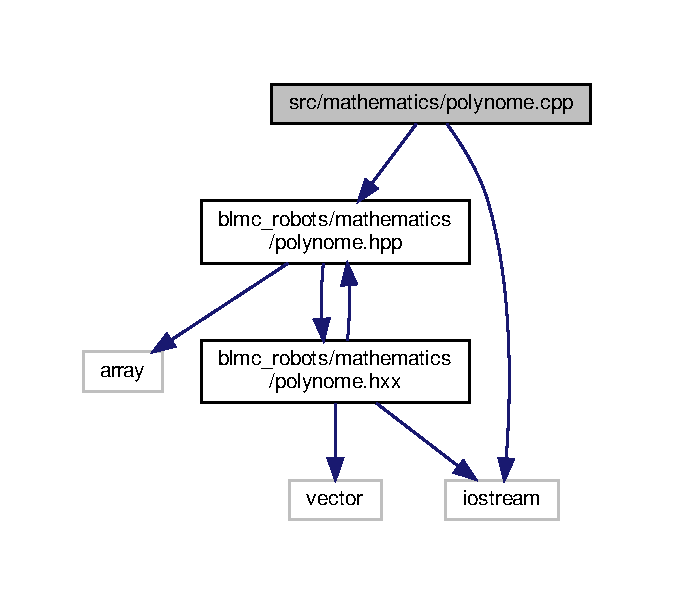
\includegraphics[width=324pt]{polynome_8cpp__incl}
\end{center}
\end{figure}


\subsection{Detailed Description}
Polynomes object for trajectories. 

\begin{DoxyAuthor}{Author}
Maximilien Naveau (\href{mailto:maximilien.naveau@gmail.com}{\tt maximilien.\+naveau@gmail.\+com}) 
\end{DoxyAuthor}
\begin{DoxyVersion}{Version}
0.\+1 
\end{DoxyVersion}
\begin{DoxyDate}{Date}
2019-\/11-\/07
\end{DoxyDate}
\begin{DoxyCopyright}{Copyright}
Copyright (c) 2019
\end{DoxyCopyright}
See \href{https://github.com/jrl-umi3218/jrl-walkgen/blob/master/src/Mathematics/PolynomeFoot.cpp}{\tt https\+://github.\+com/jrl-\/umi3218/jrl-\/walkgen/blob/master/src/\+Mathematics/\+Polynome\+Foot.\+cpp} for further enhancement. 